\section{Overview about Image Morphospecie Processing (IMP)}
The IMP was constructed to process digital image. Basically, this program look like the other applications. It include the main \textbf{menu}, \textbf{toolbar}, \textbf{main windows} and \textbf{status bar} at the end of interface
\begin{figure}[h!]
\centering
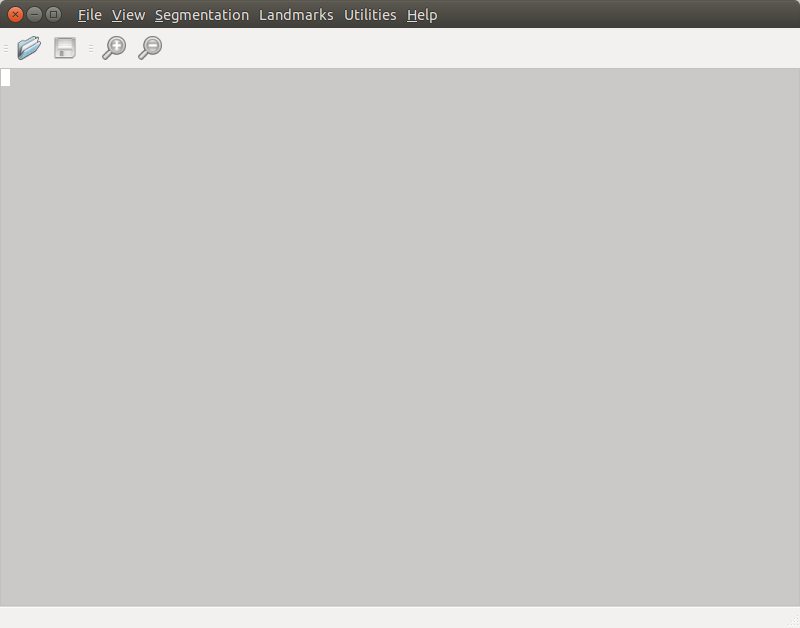
\includegraphics[scale=0.4]{images/main}
\caption{The program user interface}
\label{fig:figure_31}
\end{figure}
\subsection{Main menu}
The main menu contains all the functions of program. The functions are organized into the group followed the characteristics of functions. The main menu includes five groups described as follows:
\begin{itemize}
	\item \textbf{File} menu: contains the file's operations such as save, open, print the image or close the program.
	\item \textbf{View} menu: contains the display option of image on application 
	\item \textbf{Segmentation} menu: contains the functions to segment an image and basic methods from OpenCV
	\item \textbf{Lanmarks} menu: contains the functions to estimate and analysis the landmarks of image
	\item \textbf{Utilities} menu: contains the utility functions during processing image.
	\item \textbf{Help} menu: introduces about application.
\end{itemize}
\subsection{Toolbar and status bar}
The toolbar contains the quick access for some method in program such as: open image, save image, zoom in (25\%) or zoom out(25\%) image.\\[0.3cm]
The status bar stay at the end of program. It used to display the option value when user have change some parameter on the result.
\subsection{How to use this application ?}
The using application very easy. The user just open an image (by \textbf{File} menu or \textbf{toolbar}) then choose the correlative method.
\section{Main functions in application}
\subsection{File menu}
\textbf{File} menu provides users the functions open/save image or close program.
\begin{itemize}
	\item \textbf{Open}: open an image on program
	\item \textbf{Save}: save image to file
	\item \textbf{Save as}: save image to file with difference name
	\item \textbf{Print}: print the image
	\item \textbf{Close}: close the current window
	\item \textbf{Exit}: close the program
\end{itemize}
\begin{figure}[h!]
\centering
\includegraphics[scale=0.3]{images/menu_file}
\caption{The functions in file menu}
\label{fig:figure_31}
\end{figure}
\subsection{View menu}
\textbf{View} menu provides the solutions about display of image in program
\begin{itemize}
	\item \textbf{Zoom In}: zoom in the image 25\%
	\item \textbf{Zoom Out}: zoom out the image 25\%
	\item \textbf{Normal Size}: display image as normal size
	\item \textbf{Fit to window}: stretch the image fit to the size of windows
\end{itemize}
\subsection{Segmentation menu}
\textbf{Segmentation} menu provides the function to segment image and operations from OpenCV library.
\begin{itemize}
	\item \textbf{Edge segmentation}: extraction the edges from an image based on histogram analysis or Otsu method.
	\item \textbf{OpenCV} submenu: the basic processes on image provided by OpenCV.
\end{itemize}
\begin{figure}[h!]
\centering
\includegraphics[scale=0.25]{images/menu_segmentation}
\caption{The functions in segmentation menu}
\label{fig:figure_31}
\end{figure}
\subsection{Landmarks menu}
\textbf{Landmarks} menu provides the functions to extract and analysis the landmarks on image.
\begin{itemize}
	\item \textbf{Estimation}: estimate the landmarks of image based on difference methods, such as: edge extraction, cross-correltation.
	\item \textbf{Analysis}: analysis the estimated landmarks base on the difference methods.
\end{itemize}
\begin{figure}[h!]
\centering
\includegraphics[scale=0.25]{images/menu_landmarks}
\caption{The functions in landmarks menu}
\label{fig:figure_31}
\end{figure}
\subsection{Utilities menu}
\textbf{Utilities} menu provides another utility functions on image.
\begin{itemize}
	\item \textbf{Color 2 grayscale}: convert image to grayscale mode
	\item \textbf{Binary threshold}: apply the binary threshold to segment image
	\item \textbf{Remove yellow grid}: remove the yellow gird on image
	\item \textbf{Pairwise histogram}: compute the pairwise geometric histogram
	\item \textbf{PGH matching}: compute the measure metric between pairwise geometric histograms based on the methods (Bhattacharyya, Chi-Squared, Intersection)
\end{itemize}
\begin{figure}[h!]
\centering
\includegraphics[scale=0.3]{images/menu_utilities}
\caption{The functions in utilities menu}
\label{fig:figure_31}
\end{figure}